\documentclass[10pt]{article}\usepackage[]{graphicx}\usepackage[]{color}
%% maxwidth is the original width if it is less than linewidth
%% otherwise use linewidth (to make sure the graphics do not exceed the margin)
\makeatletter
\def\maxwidth{ %
  \ifdim\Gin@nat@width>\linewidth
    \linewidth
  \else
    \Gin@nat@width
  \fi
}
\makeatother

\usepackage{Sweavel}


\usepackage{hyperref}
\usepackage{url}
\usepackage[a4paper]{geometry}
\usepackage{a4wide}
\usepackage{float}
\usepackage[english]{babel}
\usepackage[utf8]{inputenc}
\usepackage{csquotes}
\usepackage{amsmath}
\usepackage{amssymb}
\usepackage{xspace}
\usepackage[numbers]{natbib}
\bibliographystyle{unsrtnat}
\usepackage{subcaption}
\usepackage[font={small}]{caption}
\usepackage{booktabs}
\usepackage{listings}
\usepackage{cleveref}
\usepackage{lipsum}
\newcommand{\approxtext}[1]{\ensuremath{\stackrel{\text{#1}}{=}}}
\newcommand{\matr}[1]{\mathbf{#1}}
\newcommand{\partt}[2]{\ensuremath{\dfrac{\partial {#1}}{\partial {#2}}}}
\renewcommand{\d}[1]{\ensuremath{\operatorname{d}\!{#1}}} % non-italized differentials
\newcommand{\h}[0]{\ensuremath{\hbar}} % hbar
\def\changemargin#1#2{\list{}{\rightmargin#2\leftmargin#1}\item[]}
\let\endchangemargin=\endlist 
\usepackage{amsthm}
\theoremstyle{plain}
\renewcommand{\theequation}{\thesection.\arabic{equation}}
\def\changemargin#1#2{\list{}{\rightmargin#2\leftmargin#1}\item[]}
\let\endchangemargin=\endlist    
\usepackage{xcolor}
\definecolor{Red}{rgb}{0.7,0,0}
\definecolor{Blue}{rgb}{0,0,0.8}
\usepackage{verbatim}
\def\changemargin#1#2{\list{}{\rightmargin#2\leftmargin#1}\item[]}
\let\endchangemargin=\endlist
\addtolength{\oddsidemargin}{-.35in}
\addtolength{\evensidemargin}{-.35in}
\addtolength{\textwidth}{.7in}
\usepackage{multicol}
\usepackage{graphicx}
\usepackage{epstopdf}

\epstopdfDeclareGraphicsRule{.tga}{png}{.png}{%
  convert #1 \OutputFile
}
\AppendGraphicsExtensions{.tga}

% Stephen's stuff
\newcommand{\R}{\texttt{R}}
\newcommand{\Rfunction}[1]{{\texttt{#1}}}
\newcommand{\Robject}[1]{{\texttt{#1}}}
\newcommand{\Rpackage}[1]{{\mbox{\normalfont\textsf{#1}}}}
\usepackage{xcolor}
\definecolor{Red}{rgb}{0.7,0,0}
\definecolor{Blue}{rgb}{0,0,0.8}
\hypersetup{%
  pdfusetitle,
  bookmarks = {true},
  bookmarksnumbered = {true},
  bookmarksopen = {true},
  bookmarksopenlevel = 2,
  unicode = {true},
  breaklinks = {false},
  hyperindex = {true},
  colorlinks = {true},
  linktocpage = {true},
  plainpages = {false},
  linkcolor = {Blue},
  citecolor = {Blue},
  urlcolor = {Red},
  pdfstartview = {Fit},
  pdfpagemode = {UseOutlines},
  pdfview = {XYZ null null null}
}
%% Listings
\lstset{ 
  language=R,                     % the language of the code
  basicstyle=\footnotesize,       % the size of the fonts that are used for the code
  numbers=left,                   % where to put the line-numbers
  numberstyle=\tiny\color{gray},  % the style that is used for the line-numbers
  stepnumber=1,                   % the step between two line-numbers. If it's 1, each line will be numbered
  numbersep=5pt,                  % how far the line-numbers are from the code
  backgroundcolor=\color{white},  % choose the background color. You must add \usepackage{color}
  showspaces=false,               % show spaces adding particular underscores
  showstringspaces=false,         % underline spaces within strings
  showtabs=false,                 % show tabs within strings adding particular underscores
  rulecolor=\color{black},        % if not set, the frame-color may be changed on line-breaks within not-black text (e.g. commens (green here))
  tabsize=2,                      % sets default tabsize to 2 spaces
  captionpos=b,                   % sets the caption-position to bottom
  breaklines=true,                % sets automatic line breaking
  breakatwhitespace=false,        % sets if automatic breaks should only happen at whitespace
  title=\lstname,                 % show the filename of files included with \lstinputlisting;
  % also try caption instead of title
  keywordstyle=\color{Blue},      % keyword style
  commentstyle=\color{orange},    % comment style
  stringstyle=\color{Red},        % string literal style
  escapeinside={\%*}{*)},         % if you want to add a comment within your code
  morekeywords={*,...}            % if you want to add more keywords to the set
} 

%%% Document specific
\newcommand{\course}{Structural Biology}
\newcommand{\ass}{2}
\newcommand{\term}{Lent term 2017}
%\bibliography{pga1}

%%% Title page
\title{\phantom{p}
  \bf \course: Assignment \ass \\[1em]
  \small{University of Cambridge}
}

\author{Henrik Åhl}
\date{\today}
\renewcommand{\textfraction}{0.05}
\renewcommand{\topfraction}{0.8}
\renewcommand{\bottomfraction}{0.8}
\renewcommand{\floatpagefraction}{0.75}

%%% Actual document
\begin{document}
\date{\today}
\maketitle
\setcounter{page}{1}


% \date{\today}
\phantom{a}
\maketitle
\begin{multicols*}{2}
\section*{Preface}
  This is an assignment report in connection to the \textit{\course}
  module in the Computational Biology course at the University of Cambridge,
  \term. All related code is as of \date{\today} available through a
  Github repository by contacting \href{mailto:hpa22@cam.ac.uk}{hpa22@cam.ac.uk}. 
  For all visualisations of molecules we use VMD release 1.9.3.
  
%%%%%%%%%%%%%%%%%%%%%%%%%%%%%%%%%%%%%%%%%%%%%%%%%%%%%%%%%%%%%%%%%%%%%%%%%%%%%%%
%%%%%%%%%%%%%%%%%%%%%%%%%%%%%%%%%%%%%%%%%%%%%%%%%%%%%%%%%%%%%%%%%%%%%%%%%%%%%%%
%%%%%%%%%%%%%%%%%%%%%%%%%%%%%%%%%%%%%%%%%%%%%%%%%%%%%%%%%%%%%%%%%%%%%%%%%%%%%%%
\section*{Exercises}
%%%%%%%%%%%%%%%%%%%%%%%%%%%%%%%%%%%%%%%%%%%%%%%%%%%%%%%%%%%%%%%%%%%%%%%%%%%%%%%
\paragraph*{Visulisation of complex and sequence structure\\}
  \Cref{fig:structures} shows the three complexes, 3UON, 4MQS and 4MQT in order. While 3UON is bound by antagonist, 4MQS and 4MQT are bound by acetylcholine affinity enhancing molecules. In the case of 4MQS, this is done by the agonist iperoxo, while the 4MQT structure also is bound by allosteric modulator LY2119620. Note also how the 3UON complex is stabilised with a T4-lysozyme domain, whereas the two latter are instead similarly bound by a G-protein antibody fragment. 

  \begin{figure*}[t]
    \centering
    \begin{subfigure}[H]{.33\textwidth}
      \includegraphics[width=\textwidth]{../figures/3uon}
      \caption{3UON}
    \end{subfigure}~
    \begin{subfigure}[H]{.33\textwidth}
      \includegraphics[width=\textwidth]{../figures/4mqs}
      \caption{4MQS}
    \end{subfigure}~
    \begin{subfigure}[H]{.33\textwidth}
      \includegraphics[width=\textwidth]{../figures/4mqt}
      \caption{4MQT}
    \end{subfigure}
    \caption{Molecular structures in absence of water and ions. The protein is coloured by secondary structure, while the the corresponding ligands are depicted in orange. Note how the antagonist bound structure takes on a spatially more disoriented shape, whereas the 4MQT structure, which is doubly inducing acetylcholine affinity, is similar in shape to the 4MQS complex, bound only by an agonist.}
    \label{fig:structures}
  \end{figure*}
  
  %%% Sequence / domain figures
  \begin{figure*}[p]
    \centering \phantom{h}
    \vspace{-2cm}
    \begin{subfigure}[H]{\textwidth}
      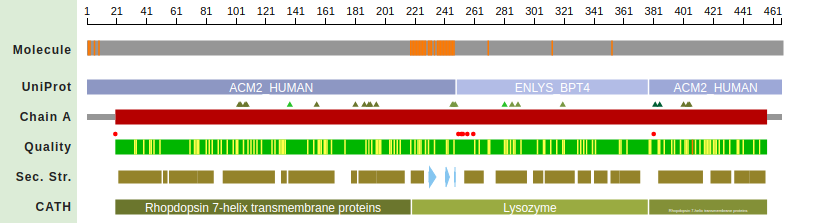
\includegraphics[width=.9\textwidth]{../figures/3uon_mutations}
      \caption{3UON}
    \end{subfigure}\\
    \begin{subfigure}[H]{\textwidth}
      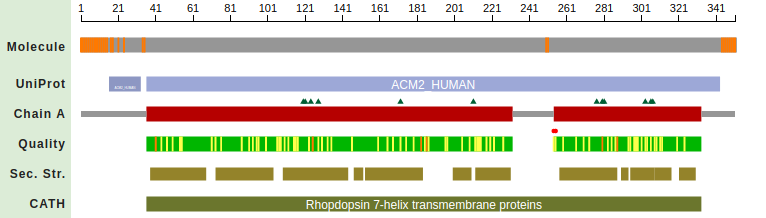
\includegraphics[width=.9\textwidth]{../figures/4mqs_mutations}
      % \caption{4MQS}
    \end{subfigure}\\
    \begin{subfigure}[H]{\textwidth}
      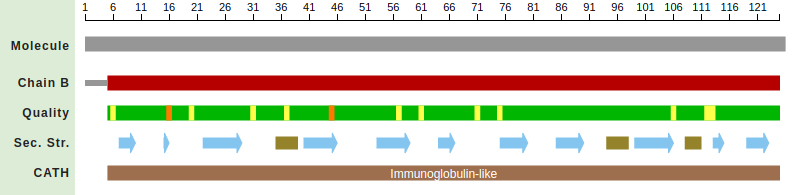
\includegraphics[width=.9\textwidth]{../figures/4mqs_macro_nano}
      \caption{4MQS}
    \end{subfigure}
    \begin{subfigure}[H]{\textwidth}
      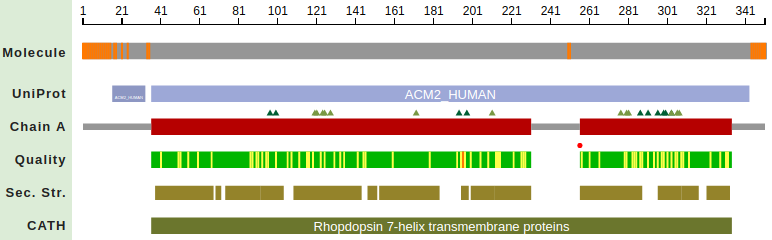
\includegraphics[width=.9\textwidth]{../figures/4mqt_mutations}
      % \caption{4MQT}
    \end{subfigure}
    \begin{subfigure}[H]{\textwidth}
      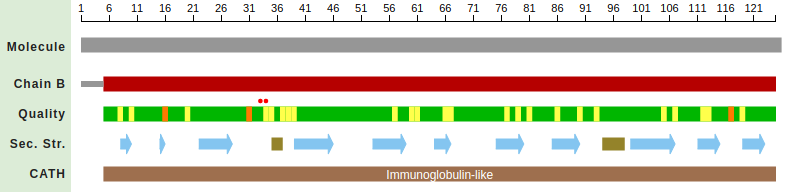
\includegraphics[width=.9\textwidth]{../figures/4mqt_macro_nano}
      \caption{4MQT}
    \end{subfigure}%
    \caption{Sequence visualisation of the three structures, separated by chain identifier. Green triangles in the \textit{Chain} identifier, describes residues involved in binding, whereas orange bars on the top row show observed mutations in various conditions. Note how mutations are primarily observed in residues not corresponding to those involved in binding, likely due to the high functional dependency of the protein on these. Indeed, for the functional molecules, mutations are only observed in intermediate domains, e.g.\ loops and the likes, which bind the helical domains together.}
  \end{figure*}
  
  For 3UON, the residues involved in binding QNB corresponds to most sites located in the region of residue id 100-195. In the other two molecules, the binding amino acids are spread out over the full region, with overlaps between the two ligand in primary sequence. Notably, the bidning sites for 4MQS and the IXO residue are not identical, even though their distribution in primary sequence view is very similar, with significant overlaps. 
%%%%%%%%%%%%%%%%%%%%%%%%%%%%%%%%%%%%%%%%%%%%%%%%%%%%%%%%%%%%%%%%%%%%%%%%%%%%%%%
%%%%%%%%%%%%%%%%%%%%%%%%%%%%%%%%%%%%%%%%%%%%%%%%%%%%%%%%%%%%%%%%%%%%%%%%%%%%%%%
%%%%%%%%%%%%%%%%%%%%%%%%%%%%%%%%%%%%%%%%%%%%%%%%%%%%%%%%%%%%%%%%%%%%%%%%%%%%%%%
\paragraph*{Summary of Haga et al.~\cite{Haga2012} and Kruse et al.~\cite{Kruse2013}\\}
  In the paper by Haga et al.~\cite{Haga2012}, the authors declare how the binding pocket we can observe part of an aqueous channel extending roughly 33 Å into the molecule from the extracellular surface. The channel itself is separated from the surface by a hydrophobic layer composed of the three amino acids LEU65, LEU114 and ILE392, which are unanimously conserved between multiple receptor subtypes (all investigated).
  
  For the 3UON structure, the QNB ligand binds deeply in the receptor pocket, and thus inhibits the response of the structure to the presence of acetylcholine. A set of aromatic amino acids forms the pocket and lid which encloses the ligand, where amino acids ASP103 (charge-charge interaction) and ASN404 (hydrogen bond) serve to orient the ligand correctly in the hydrophobic binding cavity. For reference, \cref{fig:3uon_water} shows the 3UON structure with water molecules and the ligand present. 

%%% Figure with water molecules
\begin{figure}[H]
  \centering
    \includegraphics[width=.33\textwidth]{../figures/3uon_water}
  \caption{3UON structure with water molecules (oxygen; red) and the ligand (orange) visualised. Note how the water is spread out across the structure down through the aqueous channel.} 
  \label{fig:3uon_water}
\end{figure}

\noindent
  PHE181 is also noted as involved in interacting with one of the phenyl rings on QNB, which it does downwards from the cage lid. This, however, is an interaction which is not conserved between the subtypes, and appears exclusive to the M2 complex, while other subtypes have a LEU residue in the corresponding place. 

When acetylcholine is bound, it is thought to primarily interact with ASP103 and ASN404, but it is as of yet unknown how. It might be that case that it interacts with hydrogen bonds to primarily ASN404, but possibly also to other residues.

  The authors also describe how ASP has in several mutagenic subtypes been shown as important in both agonist and antagonist binding, while mutations on ASN404 to a ALA residue has in some receptors instead been shown to significantly affect binding of the antagonist, but with little effect on the intended acetylcholine.
  
In the paper of Kruse et al.~\cite{Kruse2013}, a G-protein antibody is used instead of a lysozyme in order to stabilise the structure for imaging. In both of the molecular cases overlapping with the structures here investigated, the complex is bound by iperoxo instead of QNB. In the third case, 4MQT, the protein is also associated with a positive allosteric modulator, LYS2119620. One of the insights of the paper is how LYS2119620 binds to a pre-formed binding-site in the extracellular parts of the protein, caused by the prior binding of iperoxo. As a result of this, the outer binding pocket is contracted further. 

Like in the QNB bound protein, the iperoxo is likewise completely enclosed in the the aqueous cavity, similarly due to a lid formation of tyrosine residues, here analogously TYR104, TYR403, TYR426. In many ways, the interactions between the ligand and the protein strongly resemble those of the QNB, which the iperoxo maintains by assuming a bent conformation, and allowing for further contraction of certain parts of the surrounding backbone. In contrast to the QNB, however, there is no clear interaction with phenylalanine. ASP103 and ASN404 does however assume the same type of contact with the ligand amine, as well as direct hydrogen bonding respectively. 

When iperoxo is bound to the structure, the new complex is positively cooperational with LYS2119620, which also can activate the protein, but with lower affinity. With LYS2119620 bound, a stacking of the three aromatic rings of TYR177, TRP422, and the one found in the ligand, which is likely to enforce the binding. In addition, hydrogen bonds with residues TYR80, ASN410 and AS419 are found, as well as charge-charge interactions between the GLU172 and the LYS2119620 piperidine. Because of the location of the ligand, just above the tyrosine lid, there is also a shared interaction of the two ligands with TYR426. However, because the overall structure is largely the same between the structure bound by iperoxo and LYS2119620, and the one bound only by iperoxo, this should be indicative of LYS2119620 binding to a preformed site, caused by the association between the protein and the agonist. It is hypothesis by Kruse et al. that the additional stability in the extracellular region caused by LYS2119620 binding may also stabilise the open, active conformation of the intracellular protein.

%%%%%%%%%%%%%%%%%%%%%%%%%%%%%%%%%%%%%%%%%%%%%%%%%%%%%%%%%%%%%%%%%%%%%%%%%%%%%%%
%%%%%%%%%%%%%%%%%%%%%%%%%%%%%%%%%%%%%%%%%%%%%%%%%%%%%%%%%%%%%%%%%%%%%%%%%%%%%%%
%%%%%%%%%%%%%%%%%%%%%%%%%%%%%%%%%%%%%%%%%%%%%%%%%%%%%%%%%%%%%%%%%%%%%%%%%%%%%%%
\paragraph*{Comparison with own results}

\Cref{fig:within_5} shows the residues within 5 Å of the corresponding ligands. While we are unable to asses anything about the binding interactions themselves, we can investigate what residues are in the proximity of each other. In our case, due to the possible importance of intermediate range, weak interactions voiced by Bissantz et al~\cite{Bissantz2010}, we choose our fairly high distance. 

In accordance to supplementary information taken from the EBI PDB, we find a large overlap between our amino acids within our range and the ones stated on the database entry. This information, coupled with the investigations done by Haga et al. and Kruse et al, is shown in \cref{fig:aa_found}. As we can see, there is a large overlap between the amino acids stated as important by the paper and ours. In particular, we identify the GLU172 residue as proximal in accordance to Kruse et al -- something which the EBI PDB does not. However, as our analysis is very approximate, and does not take into account the trajectory of the molecule, it is likely that this will give more useful insights than the ones here gained. In particular, proximity does not necessarily entail interaction, and measuring for example the average distances over time for the relevant residues might yield moreo enlightening results. 

  \begin{figure}[H]
    \centering
    \begin{subfigure}[H]{.33\textwidth}
      \includegraphics[width=\textwidth]{../figures/3uon_within_5}
      \caption{3UON}
    \end{subfigure}\\
    \begin{subfigure}[H]{.33\textwidth}
      \includegraphics[width=\textwidth]{../figures/4mqs_within_5}
      \caption{4MQS}
    \end{subfigure}\\
    \begin{subfigure}[H]{.33\textwidth}
      \includegraphics[width=\textwidth]{../figures/4mqt_within_5}
      \caption{4MQT}
    \end{subfigure}%
    \caption{Isolation of ligands (coloured by atom-wise element) and amino acid (coloured by residue type) residues within 5 Ångström of the respective ligands.}
    \label{fig:within_5}
  \end{figure}

\begin{Schunk}
\begin{figure}[H]

{\centering 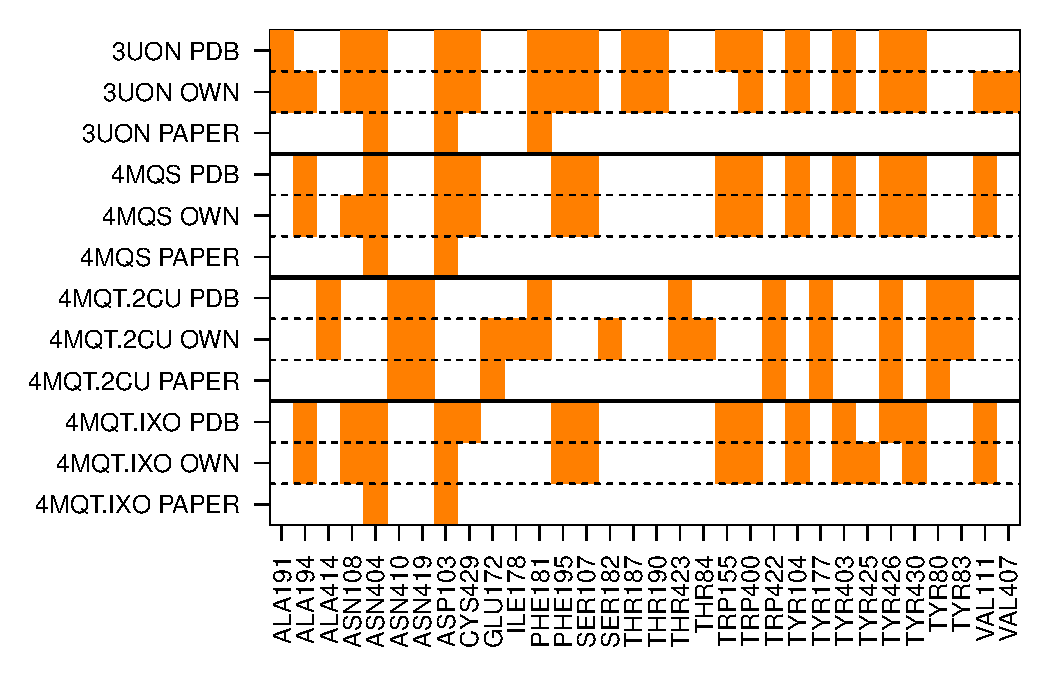
\includegraphics[width=\maxwidth]{figure/twocolumn-aa_found-1} 

}

\caption[Occurence of amino acid residue in the four different cases, with EBI PDB entry and inferred bindings mentioned by papers included]{Occurence of amino acid residue in the four different cases, with EBI PDB entry and inferred bindings mentioned by papers included. Own amino acids are taken as the ones within 5 Ångström of the corresponding ligand.}\label{fig:aa_found}
\end{figure}
\end{Schunk}


\bibliography{references}
\end{multicols*}
\end{document}
